\documentclass[11pt,letterpaper]{article}

%% ---- Packages (kept consistent with the main manuscript) ----
\usepackage[utf8]{inputenc}
\usepackage[T1]{fontenc}
\usepackage{mathpazo}
\usepackage[margin=2.5cm]{geometry}
\usepackage{graphicx}
\usepackage{float}
\usepackage{amsmath,amssymb}
\usepackage{booktabs}
\usepackage{array}
\usepackage{hyperref}
\usepackage[dvipsnames]{xcolor}
\setlength{\emergencystretch}{3em} % match main text; absorbs long \texttt{} Source paths
\hypersetup{colorlinks=true,linkcolor=MidnightBlue,citecolor=MidnightBlue,urlcolor=MidnightBlue}

%% ---- Supplementary numbering (Supplementary Table 1, 2, ...) ----
\renewcommand{\thetable}{\arabic{table}}
\renewcommand{\thefigure}{\arabic{figure}}
\renewcommand{\tablename}{Supplementary Table}
\renewcommand{\figurename}{Supplementary Figure}

\title{Supplementary Information\\[4pt]
\large Measurement and model limits of allele-specific single-cell perturbation prediction}
\author{}
\date{}

\begin{document}
\maketitle

\bigskip
\noindent This document contains the full parameter tables underlying the variant feature representation, the prediction methods and the split-half rankability analysis. Complete assignments and code are also available at \url{https://github.com/Boom5426/AllelePerturb}.

\bigskip


%% ===== Supplementary Figure 1 =====
\begin{figure}[H]
\centering
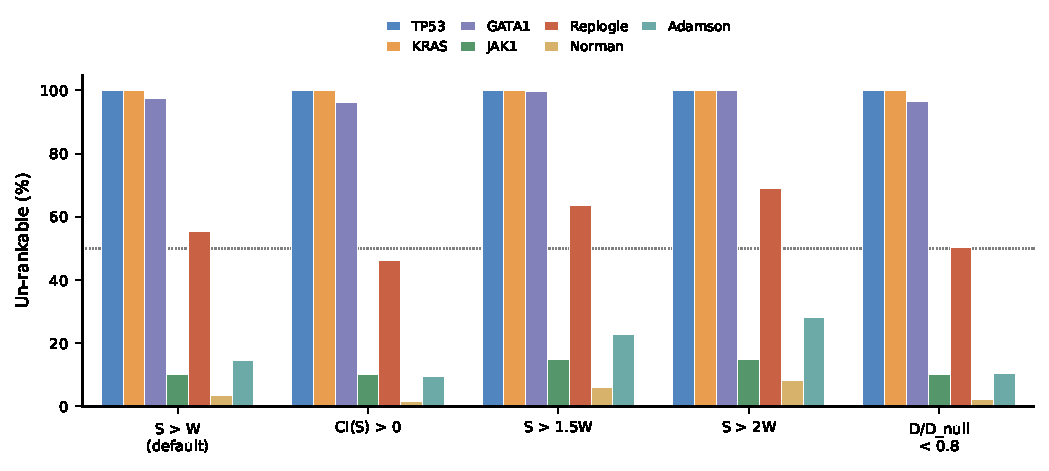
\includegraphics[width=\textwidth]{figures/ED_fig1.pdf}
\caption{\textbf{The rankability verdict is robust to the choice of criterion.} Fraction of un-rankable perturbations for the seven datasets (the four AllelePerturb genes and three gene-level Perturb-seq atlases) under five rankability criteria: the primary signal-versus-noise rule $S>W$ (default); a bootstrap lower-bound rule ($\mathrm{CI}(S)>0$, the lower $95\%$ confidence bound of $S$ above zero); two increased-stringency rules ($S>1.5\,W$ and $S>2\,W$); and a ratio threshold, under which a variant is un-rankable when $D_\mathrm{self}/D_\mathrm{null}\ge0.8$. Absolute fractions shift with stringency, but the ordering across datasets is preserved under every criterion: TP53 and KRAS remain $\sim$100\% un-rankable, GATA1 stays high, JAK1 stays low ($\sim$10\%), and among gene-level atlases Replogle is consistently the highest and Norman the lowest. Source values are listed in \texttt{results/rankability\_sensitivity.csv}.}
\label{sfig:sensitivity}
\end{figure}

\bigskip


%% ===== Supplementary Table 1 =====
\begin{table}[H]
\centering
\caption{\textbf{Variant feature ($\theta$) structural and hotspot annotations.} Per-gene residue assignments for the three structural components of the biophysical feature vector. The fold-core term $f_v$ was additionally set to $0.5$ for annotated interaction regions and $0.0$ elsewhere. The hotspot/pathogenic marker $h_v$ was defined exclusively from external prior knowledge, with no reference to the single-cell outcome.}
\label{stab:features}
\smallskip
\begin{tabular}{@{}p{1.6cm} p{3.6cm} p{2.9cm} p{5.0cm}@{}}
\toprule
Gene & Structural core ($f_v=1$) & Catalytic / switch ($s_v=1$) & Hotspot / pathogenic ($h_v=1$) \\
\midrule
TP53  & DNA-binding domain, residues 94--293 & -- & COSMIC/IARC missense hotspot codons 175, 176, 179, 220, 238, 245, 248, 249, 273, 282, 285 \\[2pt]
KRAS  & G-domain, residues 1--169 & G12, G13, Q61 & COSMIC/IARC missense hotspot codons 12, 13, 59, 61, 117, 146 \\[2pt]
GATA1 & Zinc fingers ZF1 (204--228) and ZF2 (258--282) & Zinc-finger cysteines & Zinc-coordinating cysteines 204, 207, 225, 228, 258, 261, 279, 282; ClinVar pathogenic / likely-pathogenic annotations \\[2pt]
JAK1  & Kinase domain, residues 866--1154 & -- & Functional-module membership: JH2 pseudokinase (583--855), JH1 kinase (875--1153) \\
\bottomrule
\end{tabular}
\end{table}

\noindent\textit{Note.} An earlier version of $h_v$ used the top quintile of measured effect size, which leaks the evaluation outcome into the feature; it was removed and the entire evaluation grid was re-run, with ranking performance unchanged ($\theta$-only PDS shifted by at most 0.02 and every method remained at chance).

\bigskip


%% ===== Supplementary Table 2 =====
\begin{table}[H]
\centering
\caption{\textbf{Implementation and sampling parameters.} \emph{Regression heads (top):} the six heads were crossed with three feature spaces ($\theta$, ESM, ESM+$\theta$) to form the 18 in-house feature-model combinations; all heads used a fixed random seed and were fit by minimizing squared error on the training variants. \emph{Split-half and power-analysis sampling grid (bottom):} parameters for the energy-distance split-half analysis (Fig.~4) and the depth power analysis (Figs.~4, 5), each configuration summarized by the median and the 2.5--97.5 percentile interval across seeds.}
\label{stab:heads}
\smallskip
\begin{tabular}{@{}p{4.2cm} p{3.0cm} p{5.4cm}@{}}
\toprule
Head & Family & Settings \\
\midrule
Ridge regression & Linear (L2) & $\alpha = 1.0$ \\
Lasso regression & Linear (L1) & $\alpha = 0.01$; up to 2{,}000 iterations \\
Random forest & Tree ensemble & 50 trees; maximum depth 6 \\
Gradient-boosted trees & Tree ensemble & 50 estimators; maximum depth 3; multi-output wrapper \\
$k$-nearest-neighbors & Neighbor & $k = 3$ \\
Multilayer perceptron & Neural network & hidden layers 128 and 64; ReLU; up to 500 iterations \\
\bottomrule
\end{tabular}

\smallskip
\begin{tabular}{@{}p{5.2cm} p{9.0cm}@{}}
\toprule
Sampling parameter & Values \\
\midrule
Split-half subsample sizes (per half) & 25, 50, 100, 150, 250, 400 cells \\
Representation spaces & 50-component PCA (canonical), gene space, pathway-score space \\
Random seeds per configuration & 50 \\
Power-analysis depths (per variant) & 50, 100, 150, 300 cells \\
Minimum cells for inclusion & 50 (split-half); 5 (pseudobulk profiles) \\
\bottomrule
\end{tabular}
\end{table}

\noindent\textit{Note.} Linear and neighbor heads regress directly onto the full expression profile. Because tree ensembles scale poorly to thousands of output genes, for output spaces larger than 200 genes the random forest and gradient-boosted heads were fit on a $q$-component PCA of the training profiles and predictions were mapped back to gene space by the inverse transform, with $q = \min(50,\, G,\, n_{\mathrm{train}} - 1)$.

\bigskip









%% ===== Supplementary Table 3 (decision) =====
\begin{table}[H]
\centering
\caption{\textbf{Detection, identification and prediction: a decision table for allele-specific single-cell perturbation prediction.} Three nested questions of increasing difficulty locate a dataset by its failure mode: detection (a variant versus wild type; assay sensitivity), identification (one variant versus another; ground-truth resolution) and prediction (a held-out variant from its features; computational generalization). Prediction is only meaningful once identification is achievable. Detection is graded rather than binary: in the three datasets with low measured effect size the variant-to-wild-type separation is marginal (near the replicate-noise floor; Fig.~4c,e), so `marginal' detection denotes a weak but non-zero separation from wild type. Marginal identification likewise denotes a small fraction of resolvable sibling pairs with no reliable recovery of a variant's nearest sibling. Because each gene here is also a distinct dataset, assay and cell context, a row locates a measurement and modelling regime rather than an intrinsic property of the gene.}
\label{stab:decision}
\smallskip
\begin{tabular}{@{}c c c l l@{}}
\toprule
Detection & Identification & Prediction & Limiting regime & Dataset in this study \\
\midrule
no  & --            & --            & assay-limited              & (none) \\
marginal & no        & not evaluable  & measurement-limited         & TP53, KRAS \\
marginal & marginal   & not evaluable  & measurement-limited         & GATA1 \\
yes & yes            & no             & model-limited              & JAK1 \\
yes & yes            & yes            & successful regime          & (target) \\
\bottomrule
\end{tabular}
\end{table}

%% ===== Supplementary Table 4 (published models) =====
\begin{table}[H]
\centering
\caption{\textbf{Published perturbation models under a unified allele-level evaluation.} Perturbation-discrimination score (PDS, cosine) with 95\% bootstrap confidence intervals, pooled over five generalization splits and four genes; chance is 0.50. Variant-conditionable models are scored directly; gene-keyed models are allele-blind by construction and reported by resolution coverage. Every method was scored through one harness (identical held-out variants, pseudobulk profiles, tie-aware PDS and permutation null).}
\label{tab:models}
\smallskip
\begin{tabular}{@{}p{4.2cm} p{3.0cm} l c@{}}
\toprule
Model family & Method & PDS (95\% CI) & Pearson-$\delta$ \\
\midrule
\multicolumn{4}{@{}l}{\textit{Variant-conditionable (run to completion)}}\\
Optimal-transport flow & CellFlow & 0.51 (0.48--0.54) & 0.12 \\
Attribute disentanglement & Biolord & 0.49 (0.47--0.52) & 0.13 \\
Latent arithmetic (dose) & scVIDR & 0.50 (0.48--0.53) & 0.13 \\
Latent arithmetic & scGen & 0.49 (0.46--0.52) & 0.18 \\
Conditional-flow generative & PerturbNet$^{\dagger}$ & 0.54 (0.51--0.57) & 0.13 \\
Feature regression & baselines (Fig.~2) & 0.49--0.52 & 0.55--0.65 \\
\midrule
\multicolumn{4}{@{}l}{\textit{References}}\\
Gene identity & Gene-mean & 0.49 (0.46--0.52) & 0.66 \\
No perturbation & WT-null & 0.50 & -- \\
\midrule
\multicolumn{4}{@{}l}{\textit{Allele-blind by construction (resolution coverage 4/470 = 0.85\%)}}\\
Foundation model & scGPT & n/a$^{\ddagger}$ & -- \\
Gene knowledge graph & GEARS & n/a$^{\ddagger}$ & -- \\
Virtual-cell (one-hot) & STATE & n/a$^{\ddagger}$ & -- \\
\midrule
\multicolumn{4}{@{}l}{\textit{Did not converge}}\\
Compositional autoencoder & variant-CPA & non-finite loss & -- \\
\bottomrule
\end{tabular}

\smallskip
\footnotesize $^{\dagger}$PerturbNet generates within a 50-dimensional principal-component subspace in which random predictions already score 0.52; full-space-at-chance predictors (Ridge-esm, Gene-mean) projected into the same subspace are likewise inflated to 0.52, and its exceedance over a subspace permutation null is not significant (permutation $P=0.13$). $^{\ddagger}$These models condition on perturbed-gene identity and assign an identical prediction to every variant of a gene, so an allele-level PDS is undefined (a category error).
\end{table}

%% ===== Supplementary Table 5 (per-gene backbone) =====
\begin{table}[H]
\centering
\caption{\textbf{Per-gene detection ratio, achievable ceiling and model performance.} Split-half energy-distance ratio $D_\mathrm{self}/D_\mathrm{null}$; oracle discrimination ceiling (independent second measurement, estimating attainable discrimination); fraction of allele pairs resolvable above replicate noise; fraction of variants rankable at native depth; and best in-house model PDS (canonical multi-seed harness). Chance is 0.50.}
\label{tab:window}
\smallskip
\resizebox{\textwidth}{!}{%
\begin{tabular}{@{}l c c c c c@{}}
\toprule
Gene & $D_\mathrm{self}/D_\mathrm{null}$ & Oracle ceiling (95\% CI) & Pairs resolvable & Rankable (native) & Best model PDS$^{\dagger}$ \\
\midrule
TP53  & 0.96 & 0.485 (0.445--0.525) & 0\%    & 0\%   & 0.51 \\
KRAS  & 1.00 & 0.500 (0.440--0.566) & 0\%    & 0\%   & 0.54 \\
GATA1 & 0.88 & 0.572 (0.549--0.595) & 3.8\%  & 2.4\% & 0.50 \\
JAK1  & 0.21 & 0.792 (0.742--0.838) & 78.5\% & 90\%  & 0.52 \\
\bottomrule
\end{tabular}}

\smallskip
\footnotesize $^{\dagger}$Best model is the highest-scoring in-house feature-regression head per gene under the canonical multi-seed harness (published variant-conditionable models are compared separately in Supplementary Table~\ref{tab:models}). PerturbNet is excluded; its higher per-gene values (0.53--0.54) arise from its 50-dimensional principal-component subspace, in which random predictions already score 0.52.
\end{table}


%% ===== Supplementary Table 6 (signal and noise) =====
\begin{table}[H]
\centering
\caption{\textbf{Per-profile sampling noise and between-variant signal, by gene and depth.} Each variant's cells are cut into four disjoint groups of $m$ cells: two score the replicate ceiling and two estimate the signal, so no noise realisation enters both. $\bar{\Delta}^2$ is the mean squared separation between variants after subtracting the sampling-noise term, reported unclipped with a 95\% interval bootstrapped over both variants and cell splits; it is negative about half the time when the true separation is at the floor, and clipping it at zero would report certainty the data do not carry. $P$ is a permutation test re-partitioning the half-profiles among pseudo-variants, and is conservative because the null averages five splits and the observed estimate twenty. Rows are the eligible cohort, every variant with $4m$ cells; the file also carries a fixed cohort held constant across depths, which is underpowered and is not reproduced here. Source: \texttt{results/canonical/floor\_law\_v2.csv}.}
\label{tab:signal}
\smallskip
\resizebox{\textwidth}{!}{%
\begin{tabular}{@{}l r r r l r r r@{}}
\toprule
Gene & $m$ & $n$ & $\eta^2$ & $\bar{\Delta}^2$ (95\% CI) & $\rho^2$ & $P$ & Ceiling \\
\midrule
TP53 & 25 & 98 & 37.61 & -0.051 (-0.403, +0.339) & -0.0007 & 0.581 & 0.499 \\
TP53 & 50 & 98 & 18.87 & -0.034 (-0.231, +0.156) & -0.0009 & 0.630 & 0.499 \\
TP53 & 100 & 68 & 9.39 & -0.050 (-0.162, +0.069) & -0.0026 & 0.786 & 0.497 \\
TP53 & 150 & 35 & 6.29 & -0.060 (-0.164, +0.036) & -0.0048 & 0.840 & 0.473 \\
KRAS & 25 & 92 & 37.57 & -0.095 (-0.400, +0.210) & -0.0013 & 0.686 & 0.495 \\
KRAS & 50 & 92 & 18.78 & -0.066 (-0.247, +0.108) & -0.0017 & 0.757 & 0.497 \\
KRAS & 100 & 84 & 9.39 & -0.022 (-0.138, +0.096) & -0.0011 & 0.638 & 0.498 \\
KRAS & 150 & 49 & 6.25 & +0.055 (-0.043, +0.150) & +0.0044 & 0.135 & 0.510 \\
GATA1 & 25 & 247 & 98.18 & +2.373 (+0.561, +4.170) & +0.0121 & 0.009 & 0.512 \\
GATA1 & 50 & 209 & 49.31 & +2.153 (+0.766, +3.670) & +0.0218 & 0.001 & 0.524 \\
GATA1 & 100 & 107 & 24.82 & +0.605 (-0.226, +1.486) & +0.0122 & 0.072 & 0.520 \\
GATA1 & 150 & 57 & 16.46 & +0.778 (-0.056, +1.736) & +0.0236 & 0.021 & 0.521 \\
GATA1 & 250 & 15 & 9.67 & +0.865 (+0.128, +1.700) & +0.0447 & 0.035 & 0.540 \\
JAK1 & 25 & 14 & 78.11 & +97.183 (+56.173, +126.186) & +0.6221 & 0.001 & 0.780 \\
JAK1 & 50 & 9 & 39.92 & +83.626 (+8.442, +140.473) & +1.0475 & 0.001 & 0.821 \\
JAK1 & 100 & 5 & 19.74 & +128.768 (+4.291, +205.959) & +3.2615 & 0.002 & 0.970 \\
\bottomrule
\end{tabular}}
\end{table}

%% ===== Supplementary Table 7 (depth prescriptions) =====
\begin{table}[H]
\centering
\caption{\textbf{Depth required to reach a target replicate ceiling, and where the calculator refuses.} The nearest-competitor separation belongs to the perturbations and does not change with depth while the noise falls as $1/m$, so resolution scales linearly from a pilot and the depth reaching a target is read off the calibration by inversion. The calculator returns nothing when the pilot separation's lower confidence bound does not clear zero: no finite depth recovers a separation that is not there, and a number extrapolated from noise reads as a plan. JAK1 is a check on the scaling rather than a fit, since three pilots at different depths, on different cells and different candidate sets, agree within a factor of two. Source: \texttt{results/canonical/resolution\_law\_prescriptions.csv}.}
\label{tab:depth}
\smallskip
\begin{tabular}{@{}l r r l r r@{}}
\toprule
 & Pilot & & Nearest-competitor & \multicolumn{2}{c}{Cells per group to reach} \\
\cmidrule(l){5-6}
Gene & depth & $n$ & $\rho^2$ (95\% lower) & ceiling 0.7 & ceiling 0.9 \\
\midrule
TP53 & 25 & 98 & -0.0026 (-0.0058) & refused & refused \\
TP53 & 50 & 98 & +0.0005 (-0.0079) & refused & refused \\
TP53 & 100 & 68 & +0.0019 (-0.0033) & refused & refused \\
KRAS & 25 & 92 & +0.0004 (-0.0056) & refused & refused \\
KRAS & 50 & 92 & +0.0009 (-0.0063) & refused & refused \\
KRAS & 100 & 84 & -0.0073 (-0.0133) & refused & refused \\
GATA1 & 25 & 247 & +0.0157 (+0.0027) & 62 & 232 \\
GATA1 & 50 & 209 & +0.0010 (-0.0108) & refused & refused \\
GATA1 & 100 & 107 & +0.0051 (-0.0141) & refused & refused \\
JAK1 & 25 & 14 & +0.0750 (+0.0486) & 10 & 55 \\
JAK1 & 50 & 9 & +0.1273 (+0.0910) & 12 & 65 \\
JAK1 & 100 & 5 & +0.1670 (+0.1419) & 19 & 99 \\
\bottomrule
\end{tabular}
\end{table}

%% ===== Supplementary Table 8 (both scoring axes) =====
\begin{table}[H]
\centering
\caption{\textbf{Every method on both scoring axes, each against its own permutation null.} The residual axis scores after removing a gene-shared programme computed from training variants only. Its chance level is not 0.50: WT-null, which predicts a zero vector and therefore one constant shared by every held-out variant, scores 0.524 and its permutation null is 0.524 exactly, because training variants entering the mean have their residuals shrunk toward the origin while held-out variants do not. Nulls are formed by permuting predictions across the held-out variants of a gene; intervals are 2,000 bootstraps over variants. Six methods ($^{*}$) exceed their own null at $P<0.05$, by 0.011 to 0.025. None is established: fifty permutations floor the attainable $P$ at 0.0196, four of the six sit on that floor, and twenty-five methods were tested. Source: \texttt{results/canonical/residual\_axis\_models.csv}.}
\label{tab:axes}
\smallskip
\resizebox{\textwidth}{!}{%
\begin{tabular}{@{}l r l r l r r@{}}
\toprule
Method & $n$ & PDS (95\% CI) & null & residual-PDS (95\% CI) & null & $P$ \\
\midrule
scVIDR & 308 & 0.540 (0.505--0.574) & 0.532 & 0.557 (0.522--0.590) & 0.552 & 0.118 \\
KNN-theta & 308 & 0.486 (0.456--0.518) & 0.473 & 0.555 (0.526--0.584) & 0.531 & 0.118 \\
KNN-esm+theta & 305 & 0.486 (0.456--0.516) & 0.477 & 0.554 (0.524--0.580) & 0.531 & 0.118 \\
KNN-esm & 305 & 0.483 (0.452--0.514) & 0.478 & 0.540 (0.511--0.570) & 0.534 & 0.333 \\
PerturbNet & 303 & 0.537 (0.510--0.567) & 0.519 & 0.539 (0.510--0.571) & 0.529 & 0.216 \\
MLP-theta$^{*}$ & 308 & 0.455 (0.426--0.485) & 0.449 & 0.538 (0.507--0.567) & 0.513 & 0.020 \\
scGen$^{*}$ & 308 & 0.483 (0.452--0.515) & 0.482 & 0.528 (0.498--0.558) & 0.517 & 0.020 \\
GBoost-theta$^{*}$ & 308 & 0.475 (0.447--0.505) & 0.464 & 0.528 (0.501--0.555) & 0.512 & 0.039 \\
RF-theta$^{*}$ & 308 & 0.455 (0.425--0.485) & 0.451 & 0.527 (0.498--0.554) & 0.512 & 0.039 \\
Ridge-theta$^{*}$ & 308 & 0.460 (0.431--0.489) & 0.449 & 0.525 (0.498--0.552) & 0.502 & 0.020 \\
CellFlow & 303 & 0.501 (0.471--0.532) & 0.501 & 0.524 (0.493--0.554) & 0.524 & 0.471 \\
WT-null & 308 & 0.500 (0.500--0.500) & 0.500 & 0.524 (0.493--0.554) & 0.524 & 1.000 \\
GBoost-esm+theta & 305 & 0.471 (0.442--0.500) & 0.462 & 0.523 (0.498--0.548) & 0.508 & 0.078 \\
RF-esm+theta & 305 & 0.454 (0.424--0.484) & 0.452 & 0.522 (0.495--0.547) & 0.512 & 0.196 \\
Biolord$^{*}$ & 308 & 0.497 (0.467--0.528) & 0.493 & 0.521 (0.491--0.551) & 0.504 & 0.020 \\
Ridge-esm+theta & 305 & 0.461 (0.432--0.491) & 0.454 & 0.521 (0.493--0.548) & 0.505 & 0.059 \\
GBoost-esm & 305 & 0.471 (0.442--0.499) & 0.463 & 0.516 (0.491--0.541) & 0.508 & 0.255 \\
RF-esm & 305 & 0.452 (0.422--0.482) & 0.451 & 0.516 (0.490--0.543) & 0.511 & 0.372 \\
Ridge-esm & 305 & 0.451 (0.421--0.481) & 0.453 & 0.512 (0.487--0.538) & 0.505 & 0.353 \\
Lasso-theta & 308 & 0.458 (0.427--0.487) & 0.449 & 0.510 (0.484--0.536) & 0.500 & 0.157 \\
Lasso-esm+theta & 305 & 0.452 (0.421--0.482) & 0.451 & 0.506 (0.479--0.533) & 0.500 & 0.275 \\
MLP-esm & 305 & 0.449 (0.419--0.479) & 0.450 & 0.503 (0.473--0.532) & 0.503 & 0.529 \\
Gene-mean & 308 & 0.447 (0.417--0.476) & 0.447 & 0.500 (0.500--0.500) & 0.500 & 1.000 \\
MLP-esm+theta & 305 & 0.448 (0.417--0.478) & 0.449 & 0.499 (0.469--0.530) & 0.492 & 0.176 \\
Lasso-esm & 305 & 0.450 (0.420--0.479) & 0.451 & 0.493 (0.463--0.524) & 0.495 & 0.804 \\
\bottomrule
\end{tabular}}
\end{table}

%% ===== Supplementary Table 9 (the pre-registered panel) =====
\begin{table}[H]
\centering
\caption{\textbf{The frozen criterion applied to six published perturbation screens.} The criterion, its parameters, the datasets and four predictions were fixed before any dataset was measured (\texttt{docs/PREREG\_RESOLUTION\_PANEL\_v1.md}); nothing was tuned afterwards and no dataset was dropped. Three of the six took no part in developing the criterion. Not one is benchmarkable: every screen has a far lower identifiable than detectable fraction, and the two largest atlases still order graded predictors at 0.997 and 0.96 while 0.5\% and 1.4\% of their perturbations are identifiable. One of the four predictions failed: Adamson and Replogle are reversed on the detectable fraction relative to the manuscript's own pipeline, by 3.3 percentage points, so the packaged criterion and that pipeline are not interchangeable. Source: \texttt{results/canonical/resolution\_panel.csv}.}
\label{tab:panel}
\smallskip
\resizebox{\textwidth}{!}{%
\begin{tabular}{@{}l r r r r r l@{}}
\toprule
Dataset & $n$ & Detectable (\%) & Identifiable (\%) & Ceiling & $P$(order) & Verdict \\
\midrule
McFarland & 10 & 90.0 & 20.0 & 0.928 & 0.418 & detectable \\
Tahoe-100M & 7 & 71.4 & 42.9 & 0.929 & 0.106 & detectable \\
Norman 2019 & 195 & 68.7 & 0.5 & 0.898 & 0.997 & detectable \\
Replogle 2022 & 414 & 51.2 & 1.4 & 0.865 & 0.959 & detectable \\
Adamson 2016 & 94 & 47.9 & 3.2 & 0.851 & 0.974 & not detectable \\
Virtual Cell Challenge & 139 & 25.9 & 4.3 & 0.806 & 0.903 & not detectable \\
\bottomrule
\end{tabular}}
\end{table}

\bigskip

\noindent\textbf{Supplementary Note: robustness and sensitivity controls.}

\smallskip
\noindent\textit{Statistical independence of variants.} Because some residues carry more than one substitution, the 470 variants are not fully independent. Under the random split, 47\% of held-out variants share a residue with a training variant (positional 0\%, mechanistic 10\%, low-depth 37\%, compatibility 54\%); the random split is therefore an optimistic setting, yet allele discrimination remained at chance under it and under the residue-disjoint positional split alike. Resampling residue-level clusters rather than individual variants in the bootstrap left the per-method PDS intervals essentially unchanged: all 23 non-null predictors continued to overlap the 0.50 chance level (only PerturbNet excluded it, the subspace artifact described above), and Pearson-$\delta$ remained above zero for every feature-model head. The direction-versus-ranking dissociation is therefore not an artifact of treating correlated substitutions as independent units. Source: \texttt{results/reviewer\_controls/residue\_independence\_summary.csv}.

\smallskip
\noindent\textit{Wild-type reference construction.} To test whether the detection floor reflects the variant effect or the heterogeneity of the wild-type reference, we compared, at matched depth, the variant replicate distance $D_{\mathrm{self}}$, the variant-to-wild-type distance $D_{\mathrm{null}}$ and the wild-type-to-wild-type distance $D_{\mathrm{wtwt}}$ from an independent split of the wild-type cells (energy distances, 50-component PCA space). For TP53, KRAS and GATA1 the three distances coincided ($D_{\mathrm{wtwt}}/D_{\mathrm{null}} = 0.91$--$1.09$ across 50--300 cells per half), so a variant differs from wild type no more than wild type differs from itself, and $D_{\mathrm{self}}$, which involves no wild-type cells, sits at the same level: the floor is set by the absence of variant signal relative to sampling noise, not by an inflated or heterogeneous control. JAK1 shows the contrast, with $D_{\mathrm{null}}$ eight- to thirty-fold above $D_{\mathrm{wtwt}}$ ($D_{\mathrm{wtwt}}/D_{\mathrm{null}} = 0.03$--$0.12$). The ratios are stable across wild-type sampling depth, so the floor is not a depth artifact. Source: \texttt{results/reviewer\_controls/wt\_control\_diagnostic.csv}.

\smallskip
\noindent\textit{Metric-family invariance.} The detection floor is not specific to energy distance. The split-half window ratio $D_\mathrm{self}/D_\mathrm{null}$ (50-component PCA, 50 cells per half) stayed near one for TP53, KRAS and GATA1 and low for JAK1 under all five distance families tested (energy, RBF maximum-mean-discrepancy, sliced-Wasserstein, cosine and Euclidean): TP53 1.01--1.03, KRAS 0.95--0.99, GATA1 0.90--1.04, JAK1 0.05--0.40. Source: \texttt{results/canonical/metric\_family\_floor.csv}.

\smallskip
\noindent\textit{Gene-shared versus allele-specific decomposition.} Splitting each effect as $\delta_v = \bar{\delta}_g + r_v$ apportions the measured response between a component shared by all variants of a gene and an allele-specific residual; the shared fraction is a property of each dataset rather than of the metric, at 72\% (TP53), 59\% (KRAS), 29\% (GATA1) and 51\% (JAK1). What predictors actually recover follows instead from scoring the predictions against the residual: across all 24 predictors the residual Pearson-$\delta$ lay between $-0.08$ and $0.03$, so conventional direction recovery is carried almost entirely by the gene-shared component. An oracle scored on the allele-specific residual profiles, with the gene mean taken from training variants only, stayed at the axis's own 0.524 reference for TP53 and KRAS (0.509 and 0.518), was marginal for GATA1 (0.576) and high for JAK1 (0.839), so the allele-specific residual is reproducible only where the measurement resolves sibling variants. An earlier decomposition centred on a mean that included the variants being scored and gave 0.892 for JAK1; self-inclusion in the mean makes that figure optimistic. Source: \texttt{results/canonical/residual\_axis\_ceiling.csv}.

\smallskip
\noindent\textit{Representation robustness.} Under identical splits, regression heads and scoring (single deterministic pseudobulk draw; the multi-seed convention used in the main text gives PDS 0.49--0.52), every variant representation left allele discrimination at chance while recovering direction similarly: PDS-cosine 0.458--0.473 and Pearson-$\delta$ 0.628--0.659 for the biophysical $\theta$ vector, ESM-1v, four ESM2 constructions (global, mutant-minus-wild-type global, mutated-residue and local-window) and AlphaMissense; a featureless training-gene-mean predictor reached Pearson-$\delta$ 0.66 at PDS 0.44. The scoring procedure is identical across representations, but variant coverage is not, because each representation is defined only where its input exists: AlphaMissense scores were available for 374 of the 470 benchmark variants (84 of 98 for TP53, 78 of 92 for KRAS, 201 of 254 for GATA1 and 11 of 26 for JAK1), giving 389 scored variant-by-split instances against 518 for $\theta$, 511 for ESM-1v and 497 for the ESM2 constructions. Correlations between AlphaMissense pathogenicity and measured effect size are therefore reported per gene only (Spearman $-0.08$ for TP53, $-0.05$ for KRAS and $0.09$ for GATA1); cross-gene pooling is not interpretable here, because both the pathogenicity distribution and the scale of the measured transcriptional effect differ between genes. Sources: \texttt{results/reviewer\_controls/rep\_grid\_summary.csv}, \texttt{am\_summary.csv} and \texttt{am\_effect\_spearman.csv}.

\smallskip
\noindent\textit{Oracle ceiling sensitivity.} The replicate ceiling was unchanged by depth (300-cell versus full-depth) and stayed at chance for TP53 and KRAS even for a perfect prediction scored against the benchmark's noisy pseudobulk truth (TP53 0.488, KRAS 0.490); GATA1 remained marginal (0.569) and JAK1 high. Shrinking a prediction fully to the gene mean lowered discrimination to 0.500 for every gene, so mean-shrinkage denoising does not raise the ceiling.

\smallskip
\noindent\textit{Train-only preprocessing.} Refitting the per-gene standardization on training variants and wild-type cells only (excluding held-out variants) left every gene at or below chance: per-gene PDS-cosine, all-cell versus train-only, was 0.47/0.44 (TP53), 0.49/0.50 (KRAS), 0.46/0.46 (GATA1) and 0.46/0.45 (JAK1), with direction recovery essentially unchanged (mean $\Delta$PDS $=-0.01$), so the reported all-cell standardization is conservative with respect to the null. Source: \texttt{results/canonical/leakage\_control\_summary.csv}.

\end{document}
